%!TEX root = ../main.tex

\section{Results from mean-variance optimization} % (fold)
\label{sec:mean_variance}

In \autoref{fig:mv_optimal_5}, we present the optimized weights over time in the five-factor universe (four-factor when one factor is excluded). The left hand column presents weights of factors when we consider the inclusion and exclusion of HML, while the right hand column presents weights of factors when CMA is included and excluded. The dynamic weights are based on one-week-ahead forecasts from the copula model, while the static lines represent the weights based on sample estimators of the mean-variance inputs.

Accompanying the graph, \autoref{tab:mv_model} presents average MV optimal weights based on dynamic inputs of expected returns and covariances from the copula model. This table also gives average weight differences between models, as well as a number of performance measures that are based on the realized returns. The CDB statistic is based on MV optimal weights and uses the copula model as the distribution of returns. Please note that all performance measures are calculated in-sample and are not indicative of out-of-sample investing based on a copula model; they should be interpreted only in relative terms, in order to determine how much a portfolio is impacted by the exclusion of a factor.\footnote{A similar table of performance measures and average weight differences using in-sample sample estimators of expected returns and covariances is found in~\autoref{tab:mw_mv_sample} (\autoref{app:supplementary}).}

\begin{figure}[p]
  \centering
  \footnotesize
  \begin{subfigure}{0.45\textwidth}
    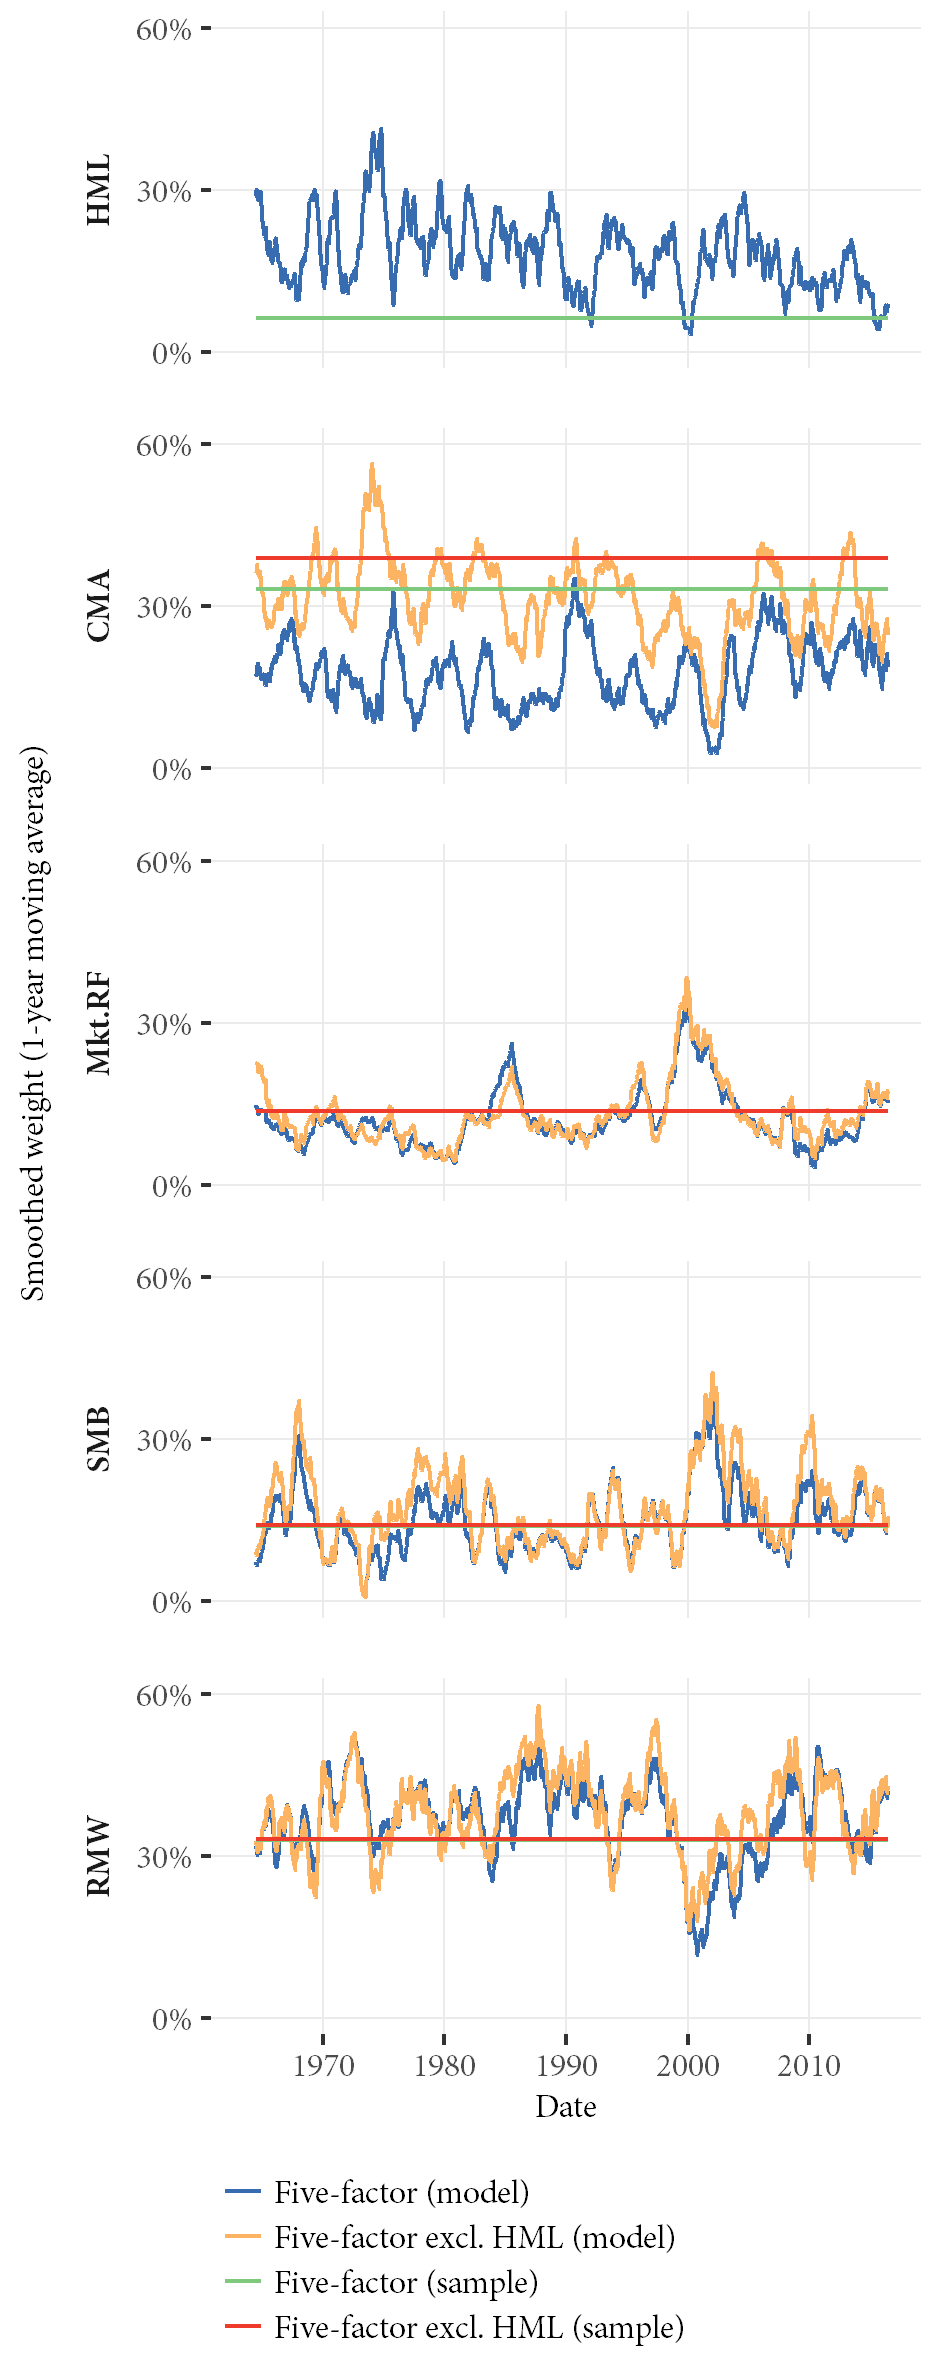
\includegraphics[width=\textwidth]{graphics/weights/main_Weights_MV_5F_EXCL_HML_5F.png}
    \caption{Excluding HML}
  \end{subfigure}
  ~
  \begin{subfigure}{0.45\textwidth}
    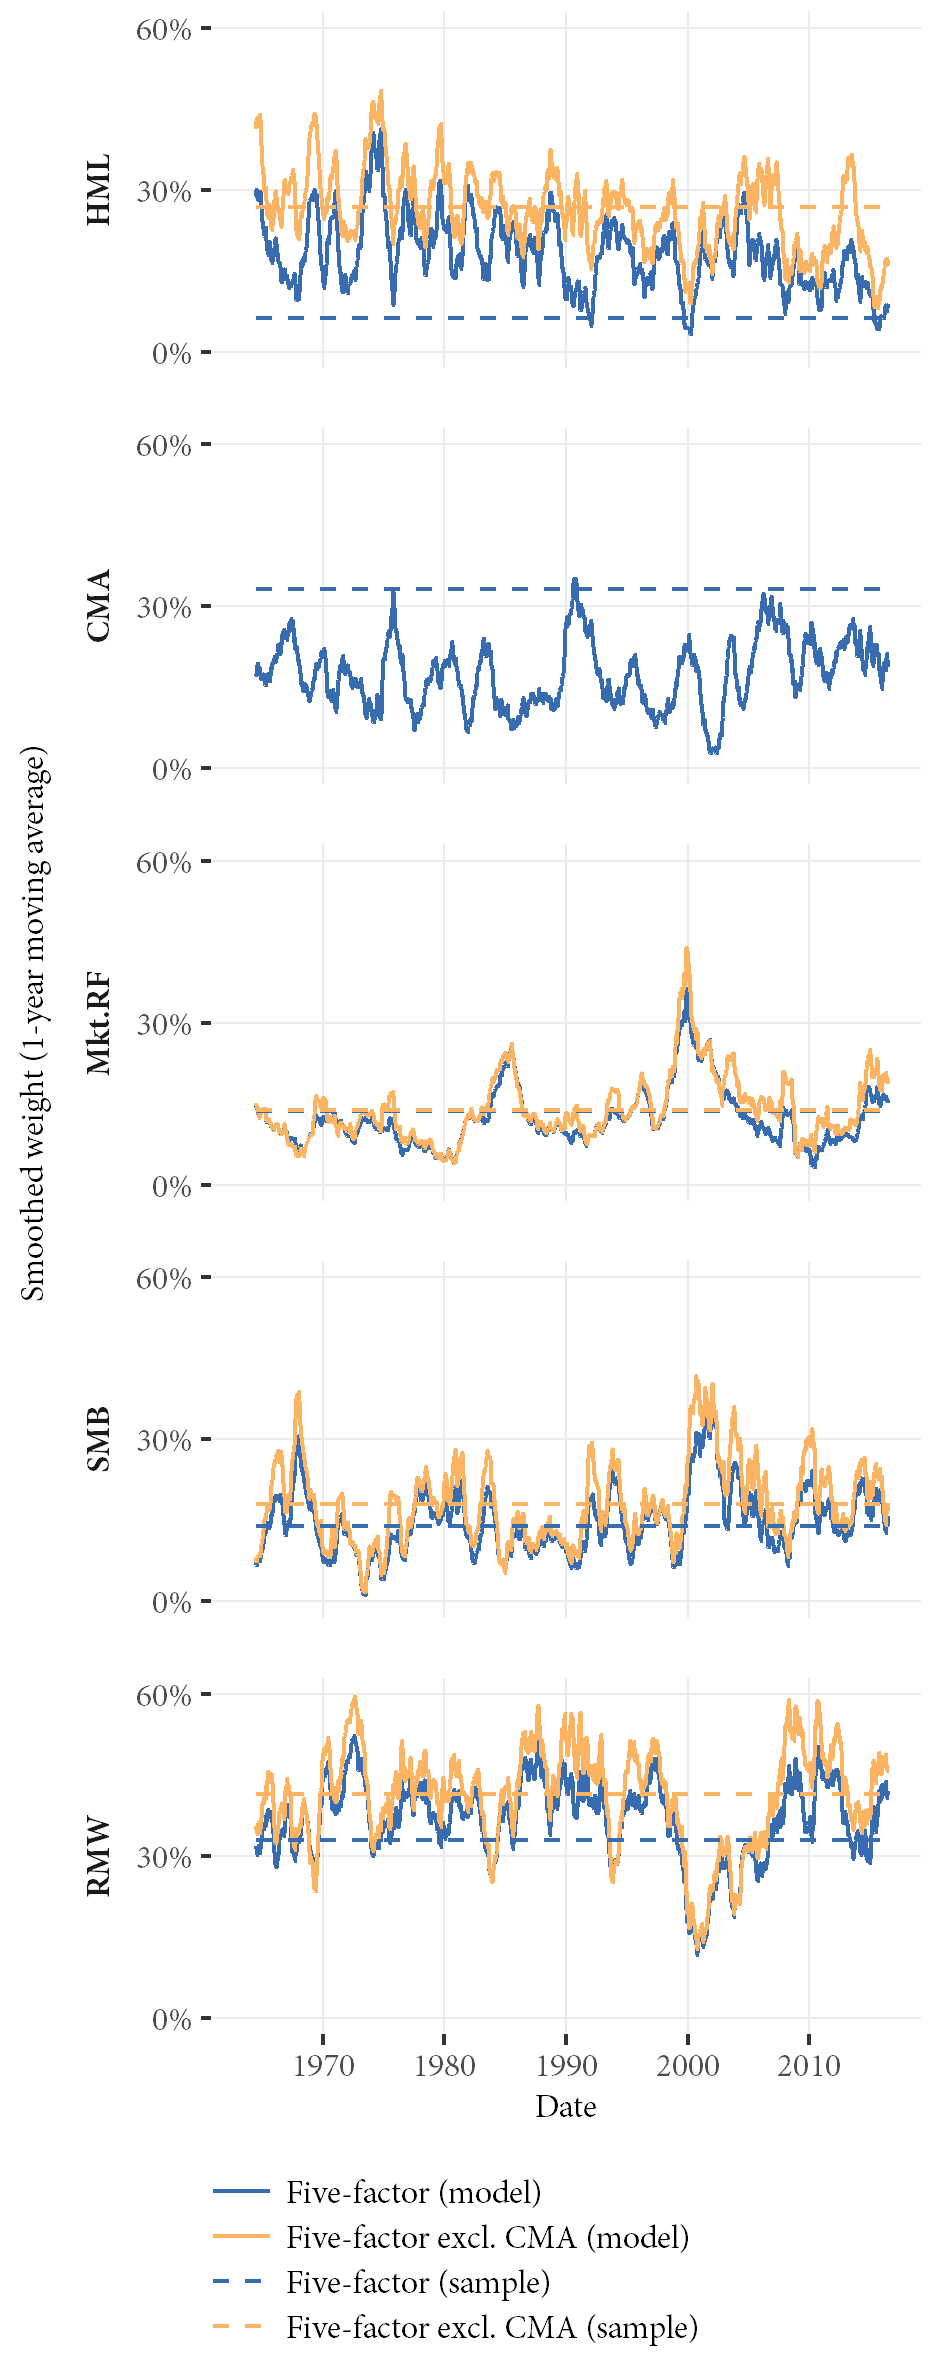
\includegraphics[width=\textwidth]{graphics/weights/main_Weights_MV_5F_EXCL_CMA_5F.png}
    \caption{Excluding CMA}
  \end{subfigure}  
  \caption{Mean-variance optimal weights with five factors}
  \label{fig:mv_optimal_5}

  \begin{longcaption}
    Smoothed as 1-year moving averages for better legibility. Optimization constrained to fully invested portfolios with non-negative weights. Left hand panel including and excluding HML, right hand including and excluding CMA. Based on one-week-ahead forecasts from the dynamic symmetric \emph{t} copula model 1963--2016.
  \end{longcaption}
\end{figure}
\begin{figure}[p]
  \ContinuedFloat
  \centering
  \begin{subfigure}{0.45\textwidth}
    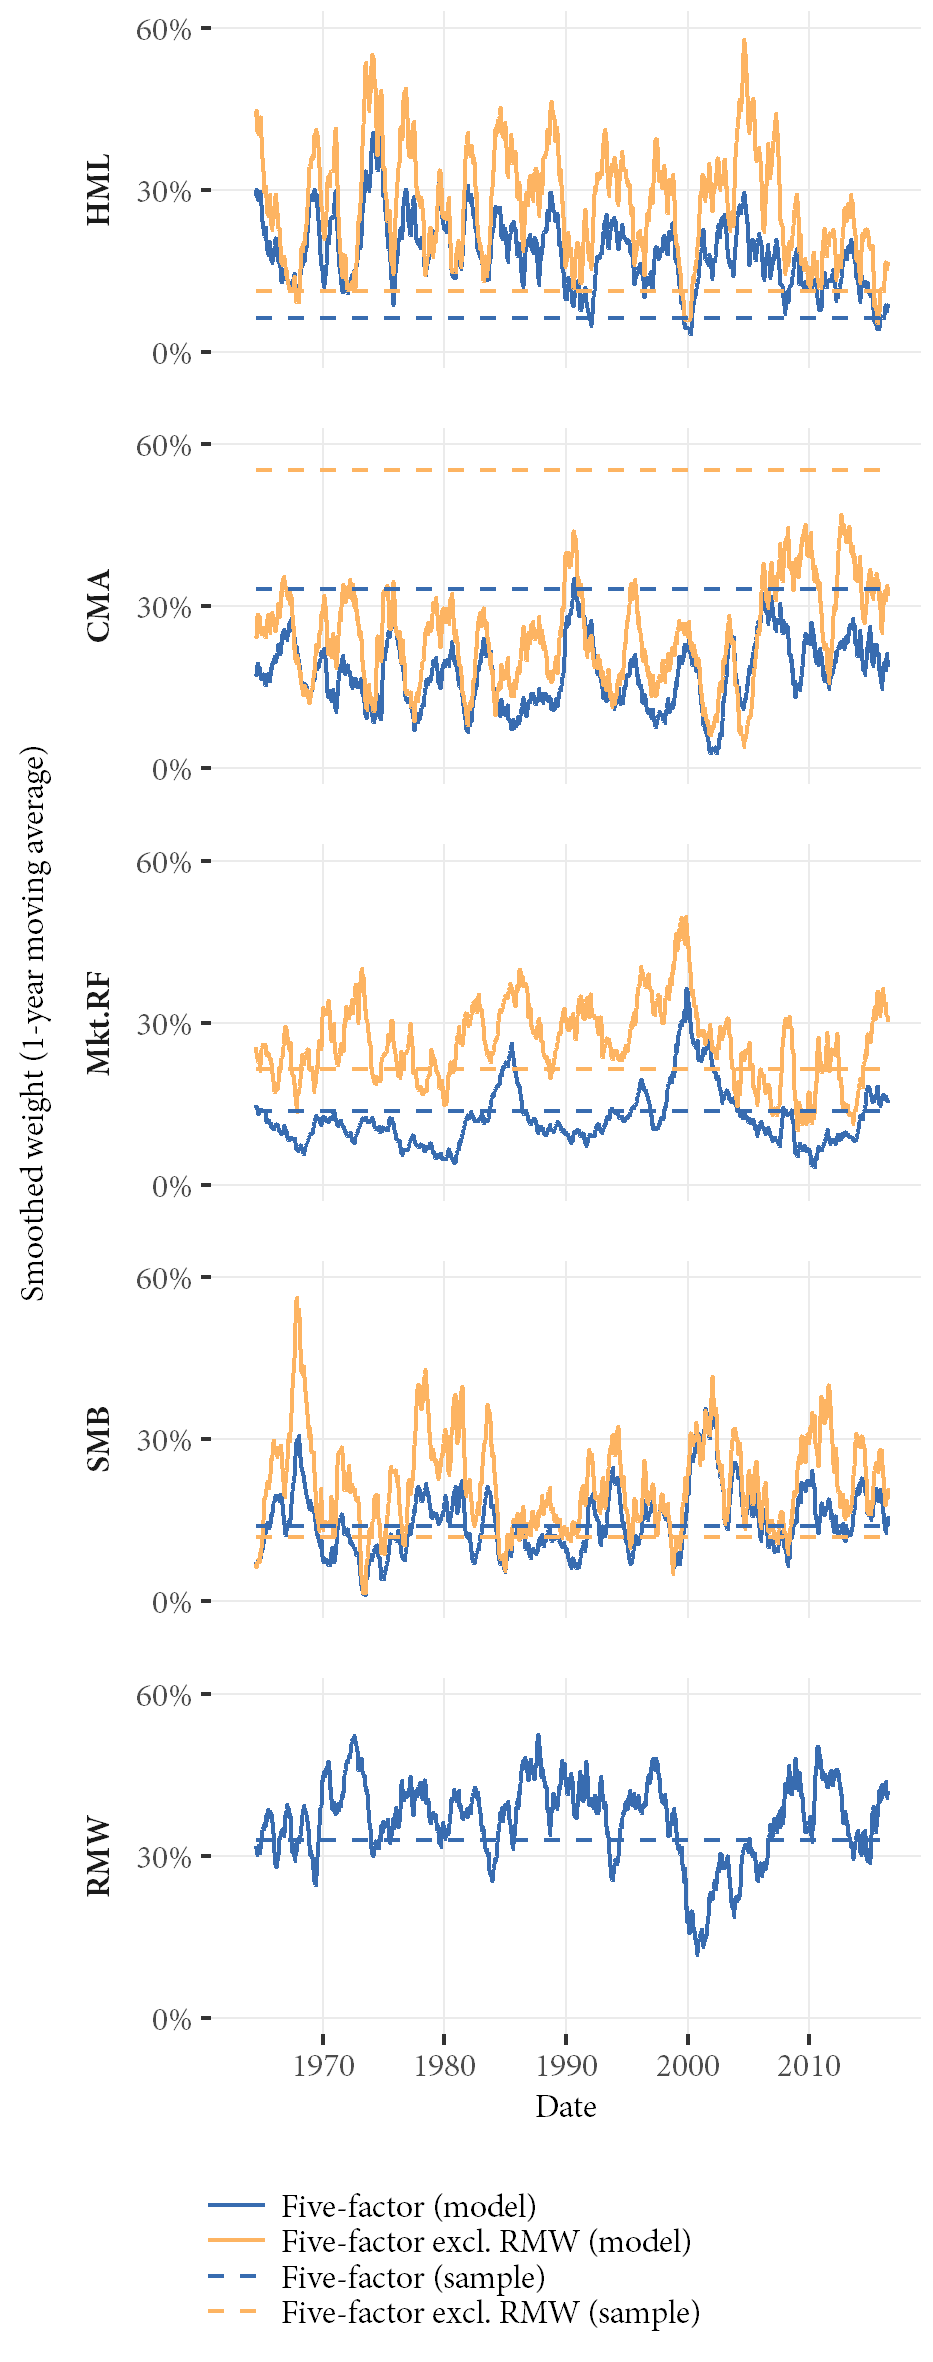
\includegraphics[width=\textwidth]{graphics/weights/main_Weights_MV_5F_5F_EXCL_RMW.png}
    \caption{Excluding RMW}
  \end{subfigure}  
  \footnotesize
  \caption{Mean-variance optimal weights with five factors (cont.)}
\end{figure}

We begin by examining the left column of plots in \autoref{fig:mv_optimal_5} that includes and excludes HML. First, we note that the weight of HML is clearly not zero when introduced in the investible universe. This appears to be the case for both the sample estimate of means and covariances, as well as the dynamic estimates from the copula model. Both inputs suggest that HML does in fact improve the tangency portfolio, as the optimal portfolio has a positive weight on the factor. The inclusion of HML leads to an increase in realized SR, which goes from 1.48 to 1.64. Furthermore, including HML leads to a less risky portfolio, with slightly lower average VaR and average ES and a higher degree of tail diversification, as measured by CDB (see \autoref{tab:mv_model}).

Although we impose the additional restriction of no negative weights, this finding does stand in contrast to the conjecture in \textcite{FF2015} that HML should not improve the tangency portfolio. While the unconstrained tangency portfolio may or may not include HML, the simple restriction of no negative weights makes HML an important part of the optimal portfolio. However, we notice that this is not recognized unless we study dynamic weights. For the full five-factor model, static sample estimators result in a lower allocation to HML (6.2\%) than the dynamic inputs from the copula (average 18.2\%), and a much smaller difference in realized SR, which goes from $1.25$ to $1.27$ (see \autoref{tab:mw_mv_sample} (\autoref{app:supplementary}) for sample results).

Second, from the left panel of \autoref{fig:mv_optimal_5}, we note that the dynamic weight of HML seems to be highly similar to the decrease in weight in CMA, while all the remaining factors seem to stay very close to their original weights when moving to the full five-factor model. In other words, the weight that is attributed to HML is drawn nearly directly from the weight of CMA, in each period. Our interpretation is that in a five-factor model excluding HML (effectively a four-factor model), CMA proxies for HML, which is why CMA absorbs nearly all the weight. HML also seems to proxy for CMA to a lesser extent, as shown by the right hand column of plots in \autoref{fig:mv_optimal_5}, which include and exclude CMA. When CMA is included, the weight of HML is lowered, but so are the weights of SMB and RMW. The proxying behavior of HML and CMA is expected, as the factors are highly correlated and zero-cost portfolio regressions in this thesis (\autoref{fig:abnormal}), as well as in \textcite{FF2015} and \textcite{Asness2015}, indicate that the main explanatory variable for HML is CMA, and vice versa.

Third, from the third panel of \autoref{fig:mv_optimal_5}, presented on a separate page, we find that among the two newly introduced factors CMA and RMW, the latter seems to have a much more substantial impact on the mean-variance portfolio. RMW receives weights of approx. 35\% in the five-factor model, which is nearly twice the allocation of any other factor. Furthermore, the inclusion of RMW leads to a large improvement of portfolio performance measures. For dynamic weights in the five-factor model, RMW makes the realized SR go from 1.28 to 1.64. At the same time, RMW leads to large decreases in the average VaR and average ES risk measures, both of which are nearly halved when RMW is included. This highlights the large benefits of including the RMW strategy in a factor portfolio, which are expected due to RMW's low or negative factor loadings in the zero-cost portfolio regressions (see \autoref{sec:alpha_reg}).

We now move on to the six-factor model universe (effectively five-factor models when one factor is excluded), with weights in \autoref{fig:mv_optimal_6} and figures in the right hand panel of \autoref{tab:mv_model}. As the optimal weights and performance results are in general qualitatively similar to the five-factor model, we will only comment on key changes.

In the expanded universe, Sharpe Ratios are generally very high, regardless of whether a factor is excluded. Surprisingly, the highest SR is realized when CMA is excluded. However, the difference is small and we do not put too much emphasis on this interpretation. Another notable change is that the allocation to HML based on static sample inputs is now higher (13.2\% compared to 6.2\%), which could be due to the clearer recognition of momentum differences between HML and CMA firms as Mom is included (cf. the discussion on zero-cost regressions in \autoref{sec:alpha_reg}). 

In summary, we examine weights and portfolio performance measures for optimal MV portfolios and find no reason to believe that mean-variance investing in the HML factor is dead or fully subsumed by the remaining factors, as the optimal portfolios include HML and have higher realized Sharpe Ratios, as well as lower realized risk measures. We also find that the inclusion of RMW is substantially more important, and leads to a large weight allocation to the factor as well as a substantial improvement on all performance measures.

\begin{figure}[p]
  \centering
  \footnotesize

  \begin{subfigure}{0.45\textwidth}

    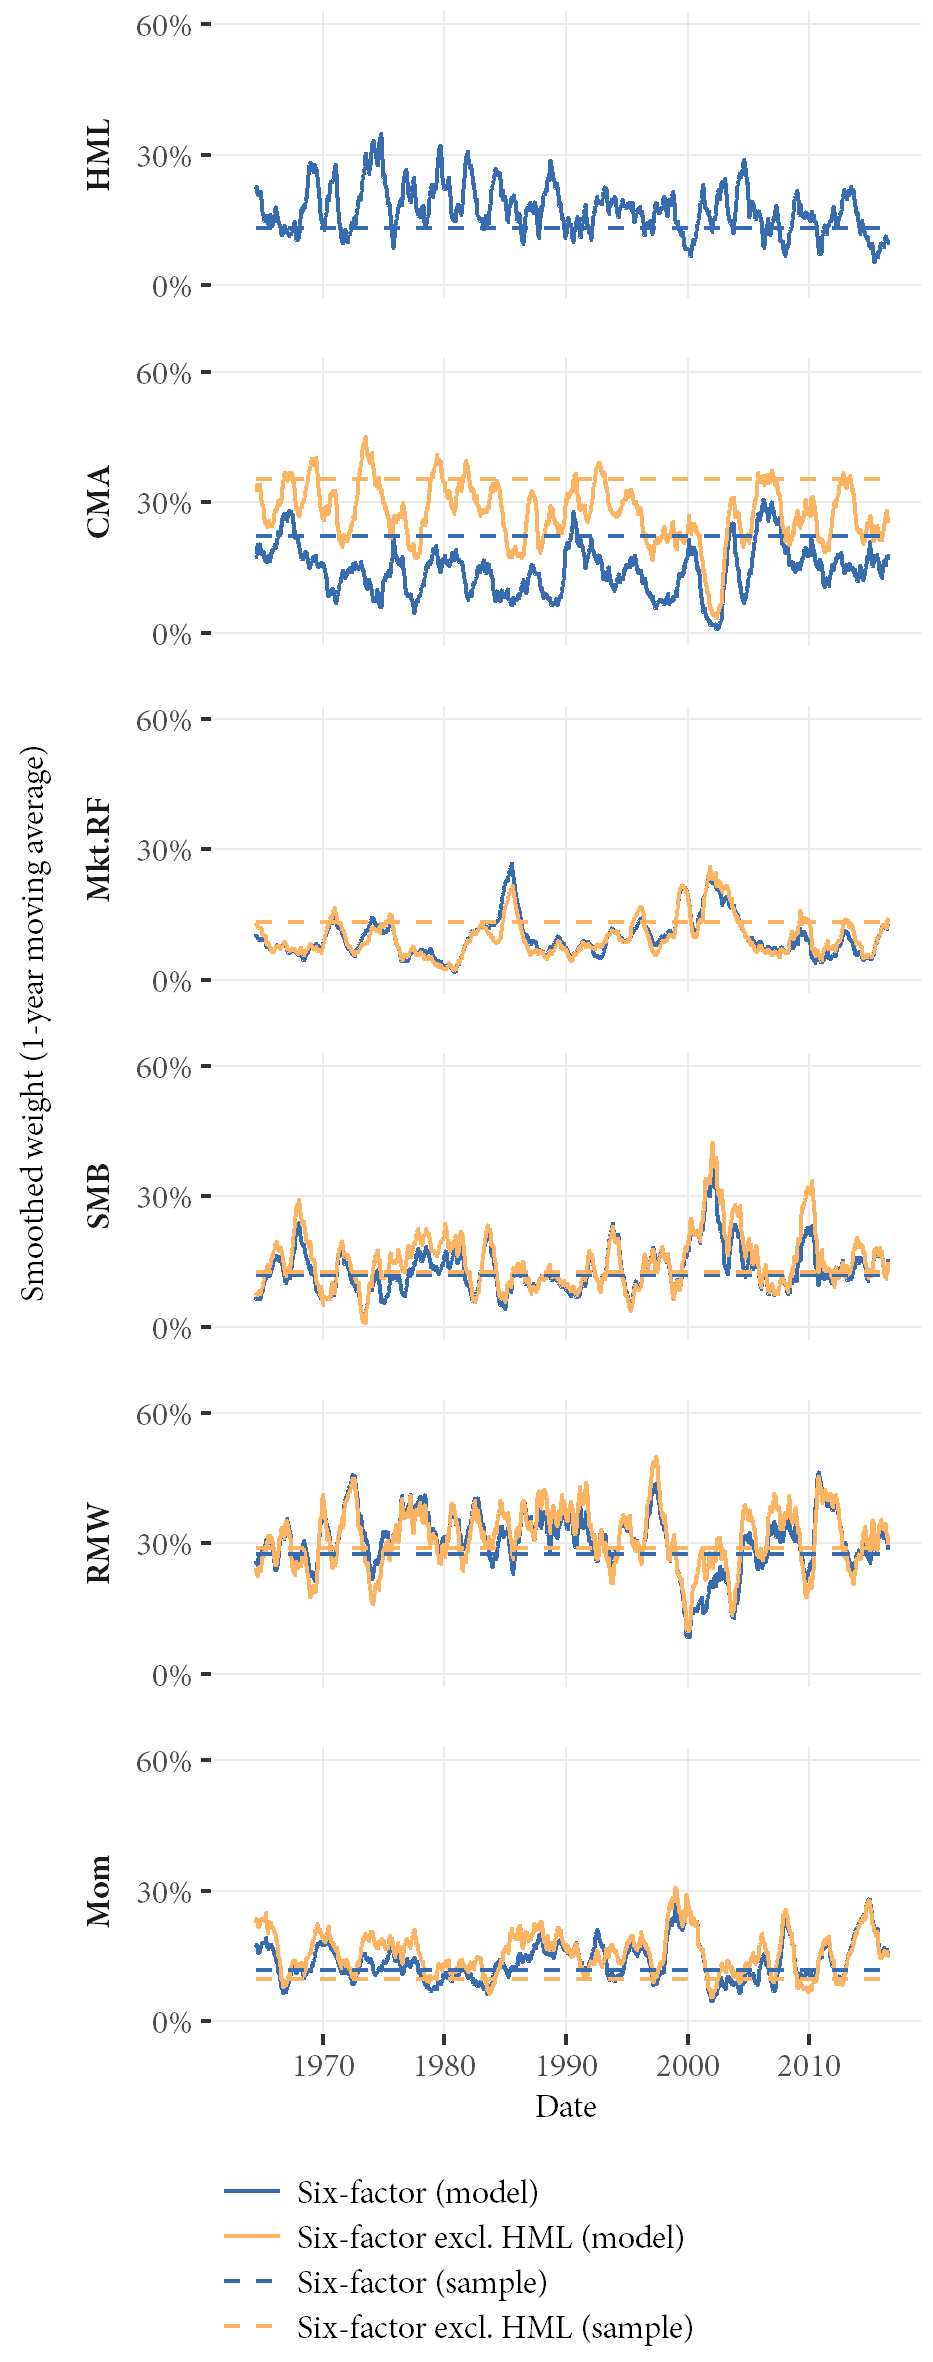
\includegraphics[width=\textwidth]{graphics/weights/main_Weights_MV_6F_EXCL_HML_6F.png}
    \caption{Excluding HML}
  \end{subfigure}
  ~
  \begin{subfigure}{0.45\textwidth}
    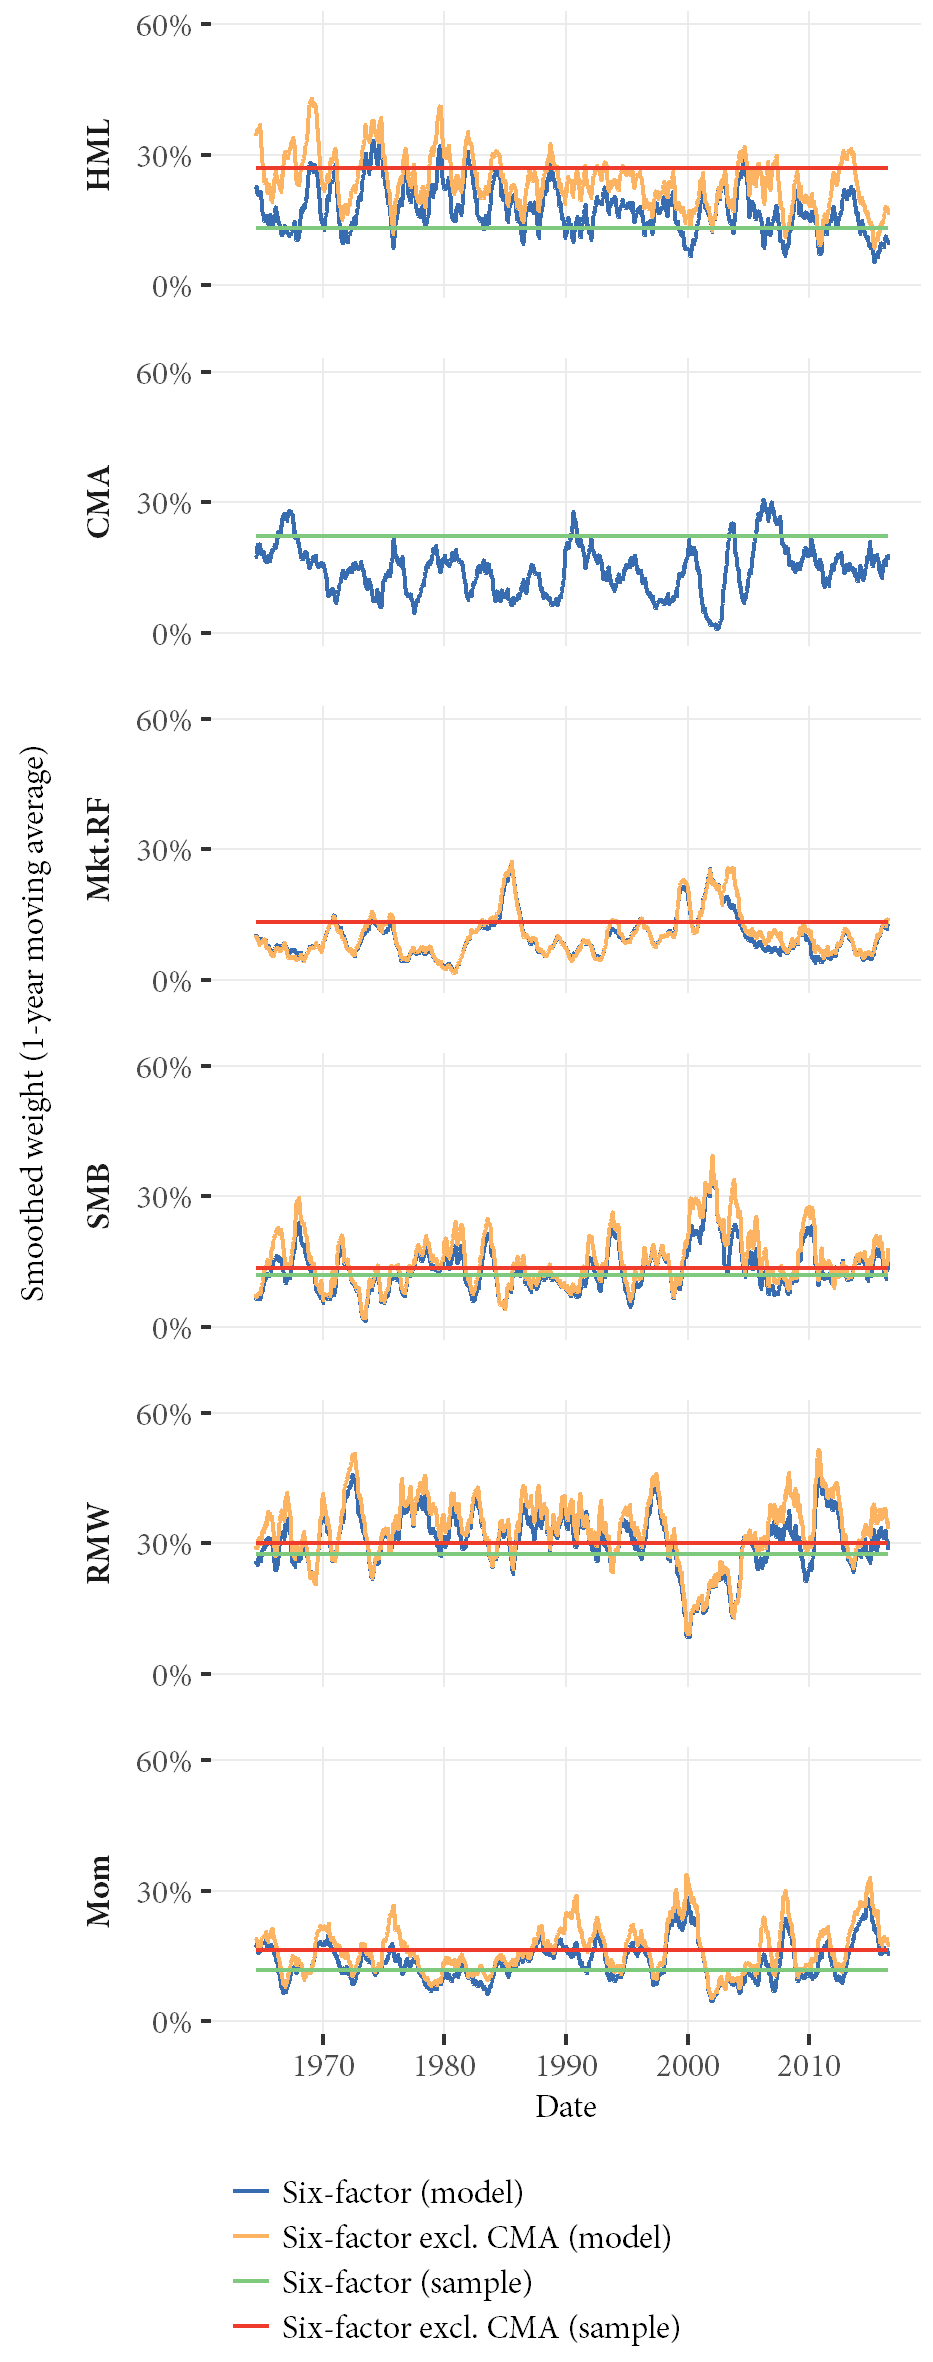
\includegraphics[width=\textwidth]{graphics/weights/main_Weights_MV_6F_EXCL_CMA_6F.png}
    \caption{Excluding CMA}
  \end{subfigure}
  \caption{Mean-variance optimal weights with six factors}

  \begin{longcaption}
    Smoothed as 1-year moving averages for better legibility. Optimization constrained to fully invested portfolios with non-negative weights. Left hand panel including and excluding HML, right hand including and excluding CMA. Based on one-week-ahead forecasts from the dynamic symmetric \emph{t} copula model 1963--2016.
  \end{longcaption}
\end{figure}

\begin{figure}[p]
  \ContinuedFloat
  \centering
  \begin{subfigure}{0.45\textwidth}
    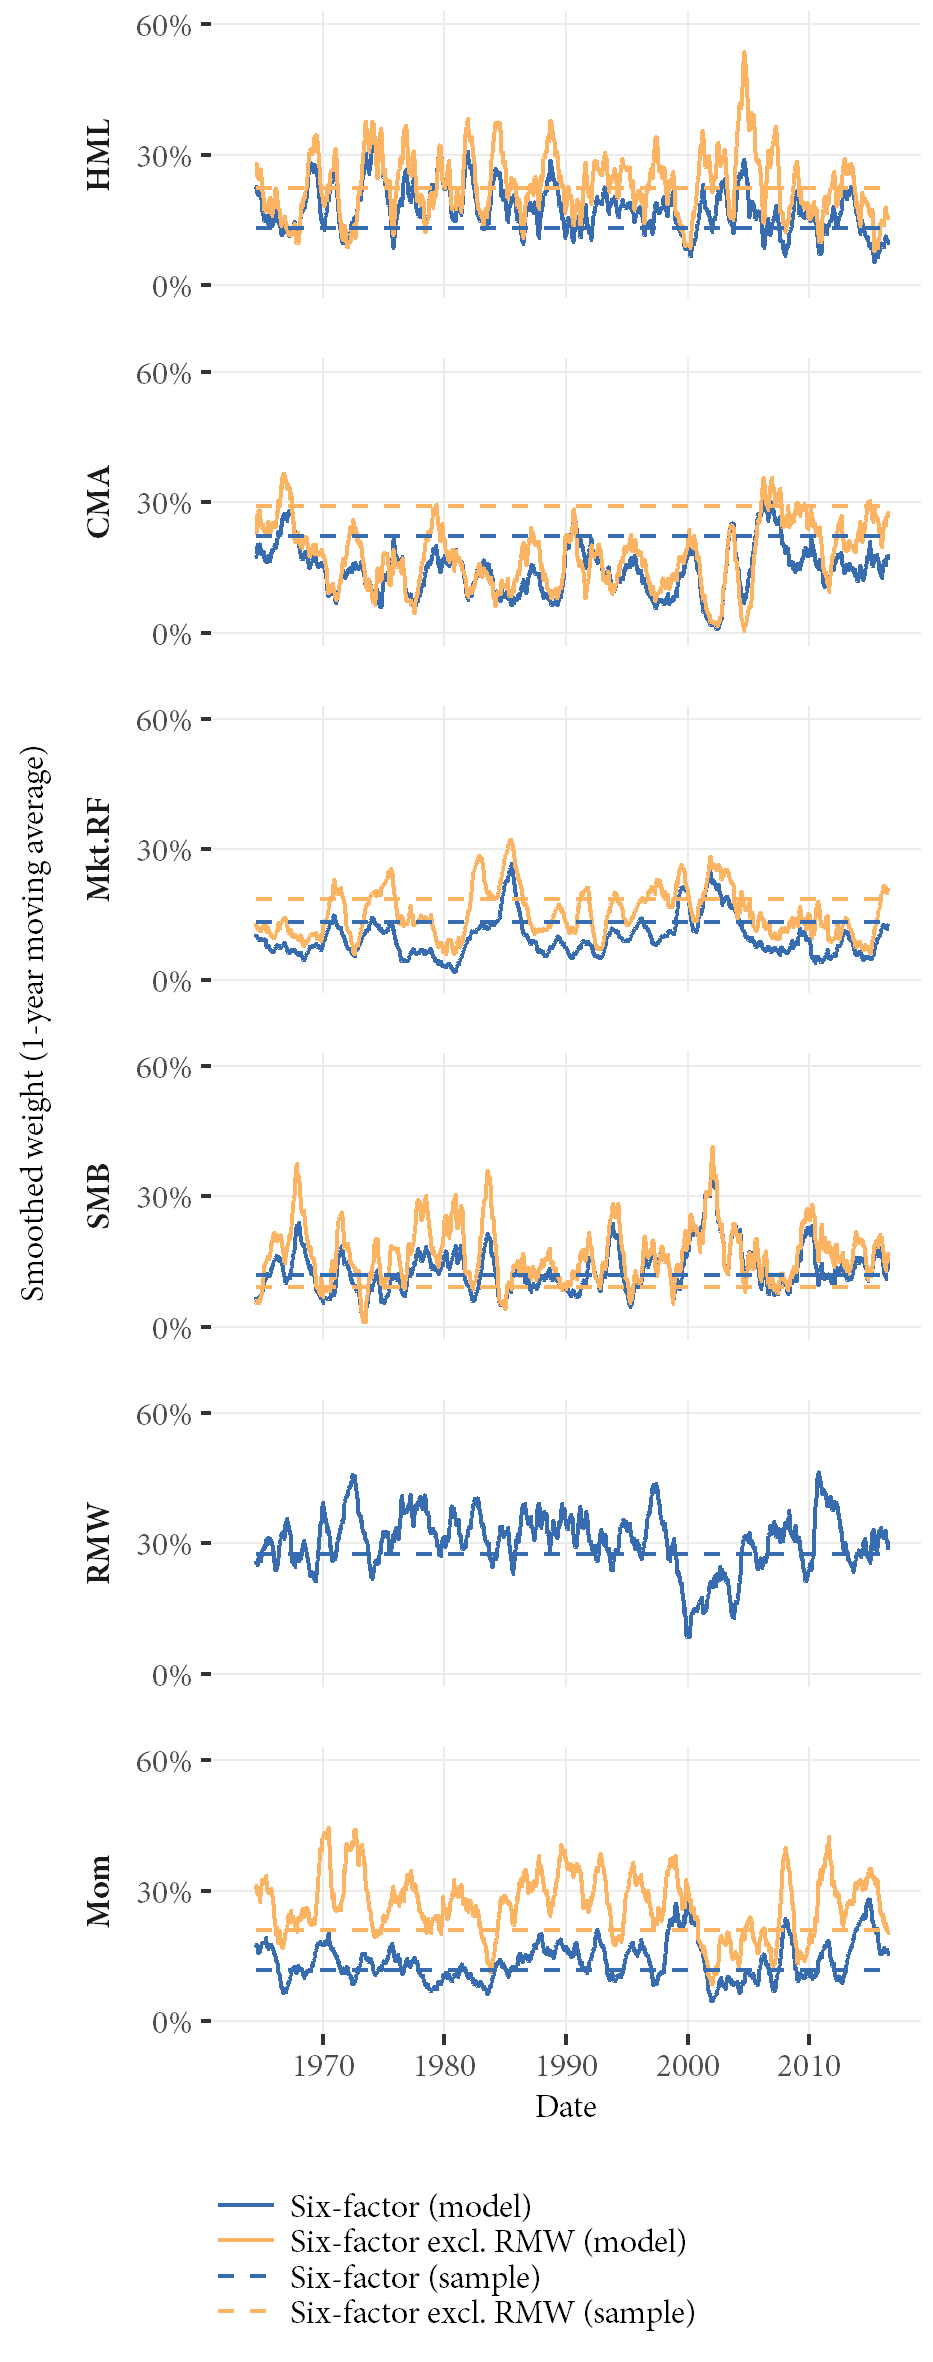
\includegraphics[width=\textwidth]{graphics/weights/main_Weights_MV_6F_6F_EXCL_RMW.png}
    \caption{Excluding RMW}
  \end{subfigure}
  \footnotesize
  \caption{Mean-variance optimal weights with six factors (cont.)}
  \label{fig:mv_optimal_6}
\end{figure}

%!TEX root = ../../main.tex

\begin{table}
  \centering
  \footnotesize
  \renewcommand{\arraystretch}{1.2}

  \caption{Mean-Variance Optimization with Dynamic Copula Model (1963--2016)}

  \begin{longcaption}
    Lorem ipsum dolor sit amet, consectetur adipisicing elit, sed do eiusmod
    tempor incididunt ut labore et dolore magna aliqua. Ut enim ad minim veniam,
    quis nostrud exercitation ullamco laboris nisi ut aliquip ex ea commodo
    consequat. Duis aute irure dolor in reprehenderit in voluptate velit esse
    cillum dolore eu fugiat nulla pariatur. Excepteur sint occaecat cupidatat non
    proident, sunt in culpa qui officia deserunt mollit anim id est laborum.
  \end{longcaption}

  \label{tab:mv_model}

  \begin{tabularx}{\textwidth}{@{} l dddd X dddd @{}}
    \toprule
    &
      \multicolumn{4}{c}{Five Factors} &&
      \multicolumn{4}{c}{Six Factors} \\
    \cmidrule{2-5}
    \cmidrule{7-10}
    &
      \multirow{2}{*}{All} &
      \multicolumn{1}{c}{Excl} &
      \multicolumn{1}{c}{Excl} &
      \multicolumn{1}{c}{Excl} & &
      \multirow{2}{*}{All} &
      \multicolumn{1}{c}{Excl} &
      \multicolumn{1}{c}{Excl} &
      \multicolumn{1}{c}{Excl} \\
    &
      &
      \multicolumn{1}{c}{HML} &
      \multicolumn{1}{c}{CMA} &
      \multicolumn{1}{c}{RMW} &&
      &
      \multicolumn{1}{c}{HML} &
      \multicolumn{1}{c}{CMA} &
      \multicolumn{1}{c}{RMW} \\
    \midrule
    \multicolumn{1}{@{}l}{\textbf{Average weights}} \\
    Mkt.RF & 12.4 & 13.2 & 14.2 & 26.4 & & 9.9  & 9.9  & 10.4 & 15.5 \\
    SMB    & 15.0 & 17.4 & 18.3 & 21.8 & & 13.4 & 15.3 & 15.6 & 16.8 \\
    HML    & 18.2 &      & 26.3 & 27.2 & & 17.6 &      & 24.1 & 23.1 \\
    CMA    & 17.6 & 31.4 &      & 24.6 & & 14.6 & 27.5 &      & 17.8 \\
    RMW    & 36.8 & 38.0 & 41.2 &      & & 30.6 & 31.4 & 33.3 & \\
    Mom    &      &      &      &      & & 13.9 & 15.9 & 16.6 & 26.8 \\
    \midrule
    \multicolumn{1}{@{}l}{\textbf{Difference weights}} \\
    Mkt.RF & & 0.8   & 1.8   & 14.0  & & & 0.1   & 0.6   & 5.7 \\
    SMB    & & 2.4   & 3.3   & 6.8   & & & 1.9   & 2.2   & 3.4 \\
    HML    & & -18.2 & 8.1   & 9.0   & & & -17.6 & 6.5   & 5.5 \\
    CMA    & & 13.8  & -17.6 & 7.0   & & & 12.9  & -14.6 & 3.2 \\
    RMW    & & 1.2   & 4.4   & -36.8 & & & 0.8   & 2.7   & -30.6     \\
    Mom    & &       &       &       & & & 2.0   & 2.7   & 12.8 \\
    \midrule
    \multicolumn{1}{@{}l}{\textbf{Performance}} \\
    Mean (\%)      & 6.48  & 6.42  & 7.28  & 8.88  & & 7.18  & 7.34  & 8.12  & 9.94 \\
    SD (\%)        & 3.95  & 4.34  & 4.72  & 6.93  & & 4.05  & 4.39  & 4.49  & 5.83 \\
    Skewness       & 0.20  & -0.22 & -0.41 & -0.20 & & -1.46 & -1.46 & -1.09 & -0.55 \\
    Kurtosis       & 13.68 & 16.13 & 15.44 & 10.36 & & 29.59 & 27.25 & 21.07 & 13.11 \\
    SR             & 1.64  & 1.48  & 1.54  & 1.28  & & 1.77  & 1.67  & 1.81  & 1.70 \\
    MDD (\%)       & 11.03 & 11.89 & 13.18 & 25.32 & & 10.48 & 11.92 & 11.19 & 13.10 \\
    Avg. VaR  (\%) & 0.59  & 0.68  & 0.73  & 1.14  & & 0.56  & 0.64  & 0.66  & 0.93 \\
    Avg. ES  (\%)  & 0.83  & 0.94  & 1.02  & 1.58  & & 0.79  & 0.90  & 0.93  & 1.31 \\
    Avg. CDB       & 0.83  & 0.79  & 0.78  & 0.68  & & 0.85  & 0.81  & 0.82  & 0.75 \\
    \midrule
    \multicolumn{1}{@{}l}{\textbf{Difference CDB}} \\
    All      & & -0.04 & -0.05 & -0.15 & & & -0.04 & -0.03 & -0.10 \\
              \\
    Excl HML & &       & -0.01 & -0.11 & & &       & 0.01  & -0.06 \\
              \\
    Excl CMA & &       &       & -0.10 & & &       &       & -0.07 \\
    \bottomrule
  \end{tabularx}
\end{table}


\FloatBarrier

% section mean_variance (end)
